%%%%%%%%%%%%%%%%%%%%%%%%%%%%%%%%%%%%%%%%%%%%%%%%%%%%
%    Harvard Data Science Review Latex Template    %
%%%%%%%%%%%%%%%%%%%%%%%%%%%%%%%%%%%%%%%%%%%%%%%%%%%%

\documentclass[]{hdsr}

%Graphics should all go in the figs/ directory
\graphicspath{{figs/}}
\usepackage[dvipsnames]{xcolor}
\usepackage{listings}
\lstset{basicstyle=\color{NavyBlue}\ttfamily,
  showstringspaces=false,
  commentstyle=\color{darkred},
  keywordstyle=\color{blue}\bfseries,
  identifierstyle=\color{black},
  stringstyle=\color{RoyalPurple},
  frame=tb,
  breaklines=true,
  postbreak=\mbox{\textcolor{red}{$\hookrightarrow$}\space},
}

\lstdefinelanguage{docker}{
  keywords={FROM, RUN, COPY, ADD, ENTRYPOINT, CMD,  ENV, ARG, WORKDIR, EXPOSE, LABEL, USER, VOLUME, STOPSIGNAL, ONBUILD, MAINTAINER, HEALTHCHECK},
  sensitive=false,
  comment=[l]{\#},
  morestring=[b]',
  morestring=[b]"
}

\begin{document}

% Larger bottom margin for the first page
\newgeometry{bottom=1.5in}

% Editorial staff will replace the following values:
% 1. Volume number
% 2. Issue number
% 3. Article DOI
% e.g. for Volume 2, Issue 3, DOI 12.345:
% \volumeheader{2}{3}{12.345}
\volumeheader{0}{0}{00.000}



\begin{center}

  \title{Using Containers to Validate Research on Confidential Data at Scale}
  \maketitle

  % Start page numbering on second page. Must appear *after* \maketitle
  \thispagestyle{empty}
  
  \vspace*{.2in}

  % Authors and Affiliations
  \begin{tabular}{cc}
    Lars Vilhuber\upstairs{\affilone,*}
   \\[0.25ex]
   {\small \upstairs{\affilone} Cornell University} \\
  \end{tabular}
  
  % Replace with corresponding author email address
  \emails{
    \upstairs{*}lars.vilhuber@cornell.edu 
    }
  \vspace*{0.4in}

\begin{abstract}
The abstract should be no more than 250 words.
\end{abstract}
\end{center}

\vspace*{0.15in}
\hspace{10pt}
  \small	
  \textbf{\textit{Keywords: }} {synthetic data; verification server; confidential data; reproducibility}
  
\copyrightnotice

\section*{Media Summary}
The Media Summary should be written in plain language to highlight the key messages of
the article, in ways that can be understood by the general public and cited by the media 
directly and accurately.  It therefore should avoid technical terms or language designed for
academic communications. It should not exceed 400 words, and more succinct, the better.

\section{A short history of synthetic data, verification servers, and improving access to confidential data}
\label{sec1}
\label{intro}

Concerns about confidentiality in statistical products have increased in the past several years. While the new disclosure avoidance techniques introduced for the 2020 United States Decennial Census \citep{abowd_2020_2022} garnered much attention, the academic community also expressed concerns about agency plans to apply formal disclosure avoidance techniques to public-use microdata files (PUMFs), and after an initial announcement, the Census Bureau delayed implementation of such methods for the American Community Survey \citep{daily_disclosure_2022}.

On the other hand, long-running pilot projects with (non-formal) synthetic microdata products (SynLBD \citep{KinneyEtAl2011}, SIPP Synthetic Beta \citep{Benedettoetal_2013}) came to an end in 2022 \citep{vilhuber_end_2022}. These pilot projects made use of a publicly accessible analysis server housing synthetic data, authorized for release in this environment by the Census Bureau and the IRS (the ``Synthetic Data Server,'' SDS), combined with a mechanism to re-run the analysis using confidential data, housed in the confidential computing environments of the U.S. Census Bureau. Researchers obtained (fast) access to the SDS, where they interactively developed their code, using the releasable synthetic data, in an environment specifically designed to mimic the Census Bureau's environment. Requests to validate the results obtained from prepared code were sent via email to designated Census Bureau staff, who then ran the code (often times debugging it), and handled disclosure avoidance analysis at the Census Bureau on behalf of the researchers. The modeling and analysis code provided by the researchers served to improve subsequent versions of the synthetic data. 

\begin{figure}
    \centering
    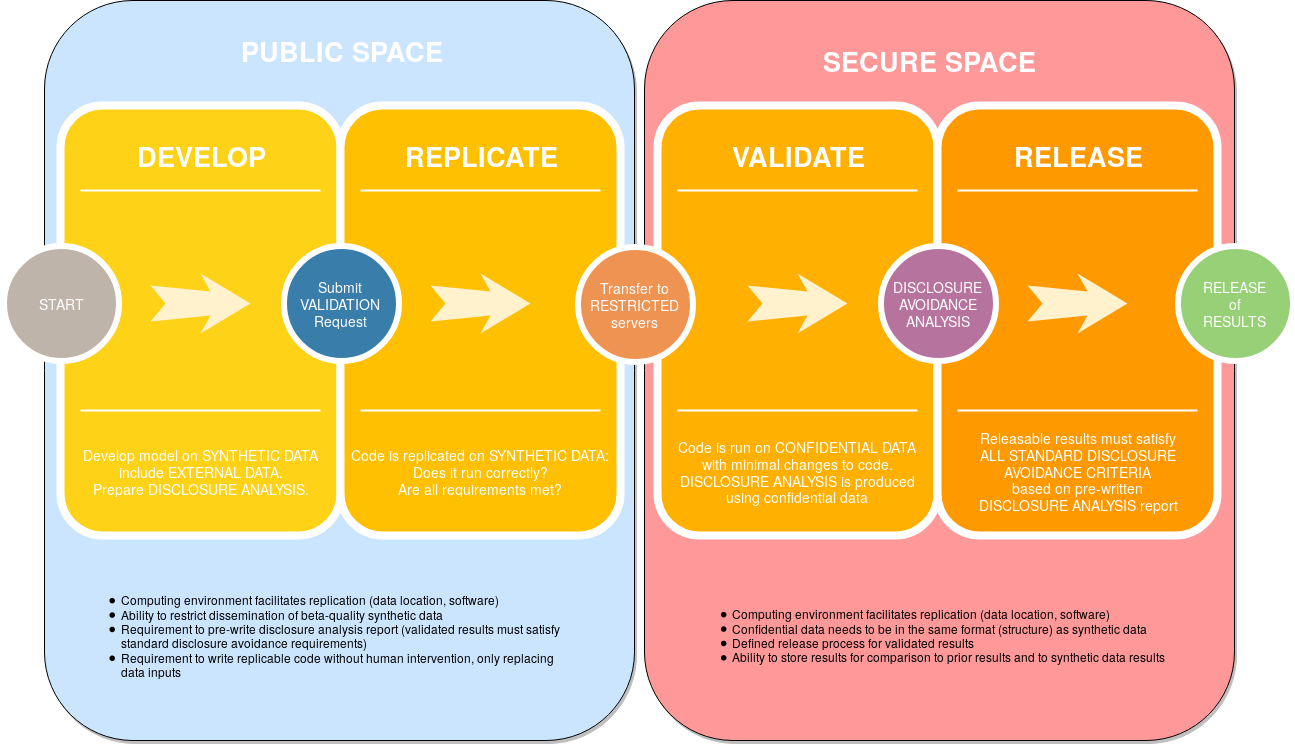
\includegraphics[width=\textwidth]{figs/SyntheticDataCycle.png}
    \caption{Processing principles of the Synthetic Data Server}
    \label{fig:data-cycle.png}
\end{figure}


\restoregeometry
\newgeometry{bottom=0.5in}


\subsection{Issues encountered with the SDS mechanism}

Code produced by researchers was often not fully reproducible, and anecdotally, the process was time-consuming for the Census Bureau staff tasked with producing the analysis on the confidential data.

\section{Scaling up access to confidential data}

If data cannot be made available due to intractable disclosure avoidance issues, yet access should be broadened, what can agencies do? 
The pilot projects described earlier were not set up to scale, and yet they demonstrated that there is a need for such a process. The number of researchers gaining access grew continuously (see Figure~\ref{fig:growth_in_sds}). Special sessions at conferences were organized around the data accessed in this fashion. In general, based on conversation of the author with various researchers at conferences and by email, researchers were happy with the ability to access such data without having to request a full-blown project in an FSRDC, but were somewhat frustrated by the process. 

\begin{figure}
    \centering
    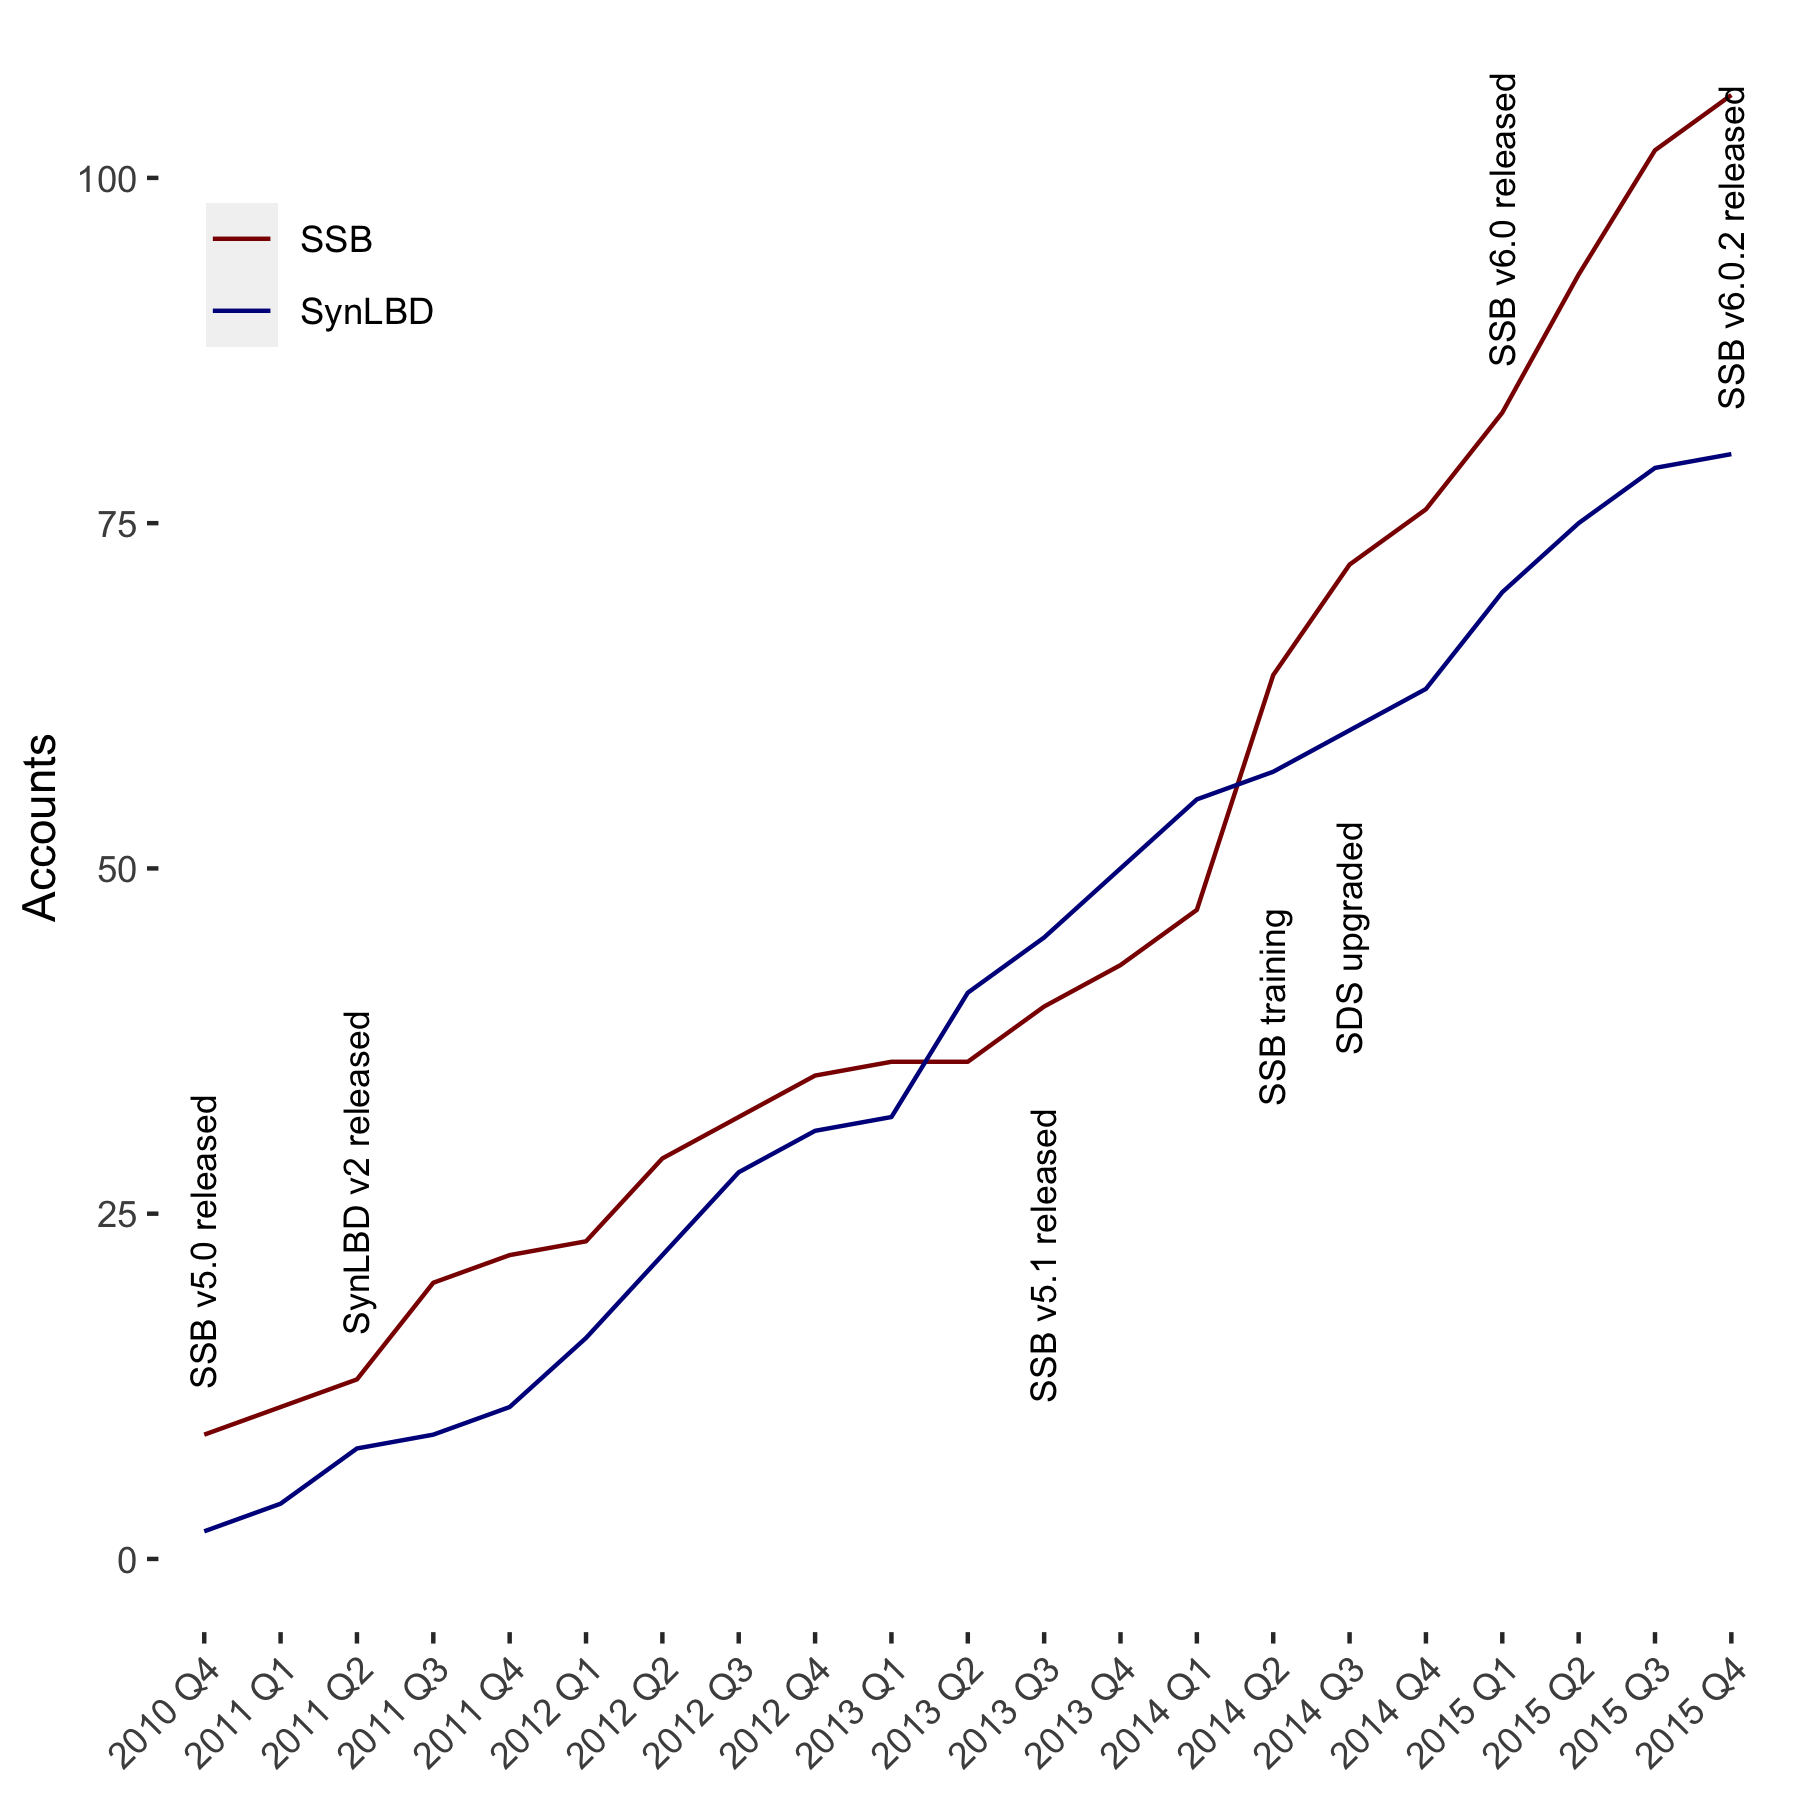
\includegraphics[width=\textwidth]{figs/accounts-2015.png}
    \caption{Computer accounts on the SDS over time}
    \label{fig:growth_in_sds}
\end{figure}

Statistical agencies and research institutes have explored various ways to scale up access to confidential data. Statistics Canada had RTRA process, Norway has the Microdata.no system, and Barrientos et al (2018) proposed a differentially private validation server. Many such processes have limitations that limit their utility for researchers. The aforementioned Statistics Canada and microdata.no systems strongly limit the type of analysis that is feasible by restricting the software keywords that can be used (RTRA), by creating a structured new statistical language (microdata.no), or by limiting the types of analysis that can be run and validated (Barrientos et al).

The issue is compounded by well-documented problems with the reproducibility of code in the social sciences. Heuristically, many of the problems with the SDS arose because the code failed to reproduce during validation, even though it was  run in a very similar environment to the development environment. Researchers in the social sciences appear to rely heavily on interactive computing, with code produced subsequently failing simple reproducibility tests. In a sample of over 8,000 replication packages associated with high-profile economics articles, only 30\% had some sort of master script.\footnote{Code run in November 2023, searching for any filename that contained the strings `main' or `master', the most common name used for control code in economics.} In part to cater to this need, remote-access or local secure access in the form of physical or virtual secure data enclaves is still the dominant - but expensive - way to access confidential data. The dominant method of access thus forces researchers to choose between lower quality data in an environment that corresponds to their preferred computing method, and higher quality confidential data in environments that are expensive for researchers, data providers, or both.


\section{A proposal using Containers}
\label{sec:proposal}
We demonstrate a simple scenario of using containers, which can be hosted on a cloud platform, but also run individually on researcher compute platforms, to facilitate synthetic and confidential data processing. The purpose of using containers is to provide users with access to synthetic data and coding resources such that their analysis is easily reproducible. Containers can easily be validated for reproducibility before they are then forwarded to the confidential computing environment. Once determined to be reproducible, extending the analysis to use confidential data, and enables a wide spectrum of plug-in disclosure avoidance measures as well. Crucially, all validation of reproducibility can be performed prior to validation using the confidential data, on open, possibly commercial platforms. Only once reproducibility is confirmed is the same analysis model ported to the confidential data. 

The use of cloud providers removes the need for users of the synthetic to install anything locally. The use of containers enforces reproducibility out-of-box when using synthetic data, as well as streamlines validation against the confidential data (which is in essence a replication of the analysis on the synthetic data). Furthermore, it enables scalability. Codeocean is a commercial service facilitating that process by making the resources available through a web browser, though the basic functionality can be achieved on any container system. Options include [Wholetale](https://wholetale.org), [Gigantum](https://gigantum.com/), and others. Finally, users who wish to not use such services can also typically provide their own setup for the synthetic data component, at very little additional cost or effort. Many university computing system provide some support on their high-performance computing clusters. For data providers, the tools used (containers) are widely used by numerous cloud providers, are transparent in how they are built, and allow for in-depth security scanning while retaining much of the flexibility that researchers and IT providers seek.

The use of containers in this way is novel as a systematic way to provide scalable, potentially high-throughput validation, and differs in usage from previous methods, such as the Cornell Synthetic Data Server. In the same 8,000 replication packages mentioned earlier, only 0.13\% had used containers. However, it has been used in a small number of well-published instances in the economics literature for precisely this kind of purpose, and uses methods that are very widespread in the computer science and statistics community \citep{boettiger_introduction_2015,moreau_containers_2023}. We believe that it is promising as a modern way of implementing validation when data are confidential.

\subsection{Details}


Reproducibility is important for synthetic data products when there
is a validation or verification process involved. In such a setting, data users will first use the synthetic
data to build and test their code for a desired analysis. Once the user is satisfied with the code used to
perform their analysis, they can request validation or verification, and their code will be run by the data provider on the confidential data. Output from the analysis on the confidential data will then have to satisfy the data provider's disclosure avoidance procedures before it can be released to the user. In the case of validation, the results from the second run on confidential data are released to the user, possibly confidentialized. In the case of a verification server, the user only receives a (non-disclosive) message indicating whether her results from the first run can be considered to be inferentially valid or not.

One problem that can arise when maintaining a validation process is that the 
computing environment on the data user’s end does not exactly match the computing environment for
the internal validation. This can lead to validation attempts that fail to run correctly or at all, which
increases the wait time for data users and the staff time involved in performing the validation at the data provider. 
In order for this process to run smoothly, the data user's code needs to be reproducible.  This ensures that the user’s code can be easily transferred and
run on the confidential data. This can be achieved by using a "container." A container collects all of the
necessary libraries, dependencies, and code needed to run an analysis in a single
package. This container can then be downloaded to any machine and used with the local system to run
the application. Crucially, container systems usually have the capability to either rebuild containers in a trusted environment, or to provide to users pre-configured secure containers that are also authorized to run in the secure area hosting the confidential data. In most cases, the core container itself does not need to be transferred, only a comprehensive recipe to build such a container.

\section{A detailed use case when using synthetic data}
\label{sec:usecase}

In this section, we walk through the process for a specific use case. The Census Bureau, data owner (custodian) of the confidential SIPP file merged with administrative data known as the SIPP Gold Standard file, makes a synthetic version of the Gold Standard file available as the "SIPP Synthetic Beta file" (SSB) \citep{Benedettoetal_2013}. The container host in the public domain is Codeocean, which provides cloud-based access to Docker-based containers (called "compute capsules"). Users log in via a simple web browser, with no install required. Crucially, Codeocean provides access to Stata and Matlab compute capsules, covering 95\% of economists' software needs. A Codeocean capsule can, however, also be used by researchers on their own workstation, as long as they have Docker installed (or a compatible container runtime) and have a Stata license. Because of the standards-based approach, it is also straightforward to exchange the configured Codeocean-generated "base image" for a security-vetted base image within the confidential environment.

In this configuration, the Census Bureau can use Codeocean to house both the synthetic dataset as well as
setup and configuration code that will assist the data user in creating code that is reproducible. The data
user can then build on the setup and configuration code provided by the Census Bureau to perform their
desired analysis. To perform the analysis on the synthetic data, users may either run the code directly on
Codeocean by paying for access to computing resources (Codeocean also provides a limited amount of
storage space and computing time for free), or they may download the compute capsule to their local
machine and use their own computing resources. When the user requests validation, the Census
Bureau can download the user’s compute capsule, securely rebuild the container (if necessary), and make minimal changes to excecute the analysis in a
secure computing environment with the confidential data. By ensuring that everything can
run within the Codeocean compute capsule using the synthetic data, it also ensures that everything can
be run within the associated compute capsule's container using the confidential data, even when the confidential data is not housed on Codeocean or any publicly accessible service.
In addition to providing a location for the Census Bureau and data users to share access to the synthetic
dataset and code, it also ensures that the analysis will run correctly for both the data user and on the
confidential data. 



\subsection{Development of code on open compute servers using synthetic data}

This repository itself is the code. The code is written in Stata, and is confirmed to run on in this compute capsule.

Basic structure ([refs](https://help.Codeocean.com/getting-started/uploading-code-and-data/paths)) imposes a strict separation between code, immutable data, and reproducible results:

- all code is under `/code`
- all data is under `/data`
- all outputs [MUST be written to `/results`](https://help.Codeocean.com/getting-started/uploading-code-and-data/saving-files), otherwise they are lost. 

Outputs are regenerated at each run, and the history of such runs can be found (for the developing user) in the right pane. When the user, at the end of the development process, requests publication of the compute capsule, only the last run is published, together with code and data.

To facilitate this file organization for the user, the template code includes a [config.do](config.do) file, which applies best programming practices by defining some global variables for file paths that are used elsewhere in the code. It also instantiates logfiles, which are also written to `/results`.


%## The use of external packages

Stata, R, and many other programming languages use external packages of code to augment native capabilities. Initially, these need to be installed over the internet. However, there are various ways to address the issue at subsequent installations:

1. Packages can always be re-installed from source
2. Packages can be installed by a programming-language specific install script, and stored locally. 
3. Packages can be incorporated into the container image itself.

Codeocean has the ability to do the third method, via a "post-install" script and environment setup (see [here](https://help.Codeocean.com/getting-started/the-computational-environment/using-the-postinstall-script-for-further-customization) and [here](https://help.Codeocean.com/tips-and-tricks/language-specific-issues/using-stata-on-code-ocean)). It can also support the first method during runtime (while connected to the internet). Because each run of Stata is transitory, there is no easy way to accomodate the second method. 

We note that while hosted on Codeocean, the same image, once built, is re-used, and packages are not re-installed. However, when exporting a capsule, only the build script is exported, and a replicator would need to rebuild the container, thereby also re-installing any packages. This can lead to version discrepancies when packages cannot be pinned to a particular version (as is the case with Stata). 

\subsection{Validating reproducibility}

In its base configuration, Codeocean signals to researchers the successful completion of a run of the controller script `run` in the right pane of the user interface, indicating to the custodian of the confidential data that the code is verified to execute on the synthetic data. This is important for scalability and efficiency, as it reduces the need for extensive debugging.

\subsection{Concrete example: Estimating economic returns to education in the SIPP}

This example runs a Mincer equation on the SIPP Synthetic Beta data (need cite). The code is split into 4 pieces, tied together by a script. The environment is specified through a Dockerfile. 

% ### Script

% The script [run](run) ties all Stata programs together. An alternative would be to have both a generic run, plus a master Stata do file. Both options work.

% ### Stata programs

% - [config.do](config.do) creates various global variables, and initializes a per-program log file, which will show up in `/results`.
% - [00_setup.do](00_setup.do) initializes the code setup for each run. 
%   - It could also install Stata packages from SSC (see discussion above).
% - [01_stats.do](01_stats.do) computes a few simple descriptive stats. Only log output is generated, but this could generate a summary stats table ("Table 1") of a paper.
% - [02_mincer.do](02_mincer.do) does data prep and runs a Mincer regression. Output is generated through `esttab`, and stored in `/results/mincer_results.csv`.



\subsubsection{Dockerfile}

The Dockerfile in this case specifies the use of a Codeocean-specific pre-built Stata container, and handles installation of any Stata packages:

\lstinputlisting[language=docker,caption={Example Dockerfile},breaklines=true,label={code:dockerfile1}]{dockerfile.1.txt}

\subsubsection{Executing code on public (synthetic) data using commercial infrastructure}

Once the user has developed all the code, they execute a "reproducible run" on CodeOcean. This ensures that all code executes without error (note that it does *not* ensure that all necessary code has run - code can be commented out or be non-functional). This particular example, when run on CodeOcean infrastructure in 2021, takes about 4 minutes to execute.

\subsubsection{Executing code on public (synthetic) data using private or academic infrastructure}

Alternatively, the user can export the entire capsule (including data), rebuild the image locally, and execute on their local infrastructure, using an unmodified Dockerfile.

\lstinputlisting[language=bash,basicstyle=\footnotesize\color{NavyBlue}\ttfamily,,caption={Building the container},label={code:build}]{docker-build.txt}
%
Note that the image built has been posted publicly at \url{https://hub.docker.com/r/larsvilhuber/ssb-demo}.


\subsubsection{Validating researcher-provided code}

Should the data custodian have doubts about the verified run of the capsule, or the capsule was not validated on Codeocean (because run on private infrastructure), the replicator can run the container again, using the synthetic data. This can happen in an unsecure environment, outside of the confidential data environment, since no additional data requirements need to be satisfied.



\lstinputlisting[language=bash,basicstyle=\footnotesize\color{NavyBlue}\ttfamily,,caption={Running the container},label={code:run}]{docker-run.txt}

which runs for about 3 minutes on a 2021-vintage Linux workstation. 




\subsubsection{Porting to confidential compute server}

In order to conduct a validation exercise, the code needs to be re-executed in the secure data environment. The compute capsule is exported (via "Capsule -> Export"), which provides a full package. Since exporting the package is done here by the data owner, exporting the data is not necessary, making for a light package. Alternatively, the code can also be downloaded via `git clone` from the default CodeOcean git repository, or from a researcher's git repository. Note that it is not necessary to publish the CodeOcean capsule or to make a git repository publicly viewable, as long as it is shared with replicator.

\subsubsection{Dynamic code provided by data custodian}

As configured in the present example, the code requires only minor modifications to work on confidential data. The data custodian can provide a `config.do`  that can handle switching from synthetic to confidential for specific code pieces (Listing~\ref{code:config.do}).

\lstinputlisting[language=stata,wrap,caption={A dynamic configuration file},label={code:config.do}]{config.do}

Alternate methods exist as well. For instance, one could test for presence of "`config-confidential.do`" and include it if present, overriding any parameters in the main `config.do`.

\subsection{Modifying the container base image}

The CodeOcean capsule uses a CodeOcean-specific prebuilt container used to execute the code (in the case of this capsule, \url{registry.codeocean.com/codeocean/stata:16.0-ubuntu18.04}). This image will need to be replaced with a container that satisfies the data owner's security requirements, while maintaining full compatibility with the needs of the environment. Because this example uses Stata, which behaves fairly uniformly across various Linux installs, the particular version of the Linux base image is likely not important.   Alternatively, the validation exercise can be coordinated with the provider, and the provider can offer a generic security-vetted image that is verified to be functionally equivalent to the image used in the secure environment. Finally, the Docker file underlying the \texttt{stata:16.0-ubuntu18.04} image, which builds the container from scratch, can be used to rebuild a container within the secure environment.\footnote{\href{github.com/AEADataEditor/docker-stata/releases/tag/stata16-2021-06-09}{https://github.com/AEADataEditor/docker-stata/releases/tag/stata16-2021-06-09} for an example.} At scale, this would simply use a similar, security-vetted, pre-built container, e.g., \url{registry.census.gov/codeocean/stata:16.0-ubuntu18.04-secure}.\footnote{This is a fake URL, no such registry currently exists}

The key feature here is that no binary code needs to be transferred into the secure environment, eliminating a security risk. The execution environment is completely known to the IT personnel of the data provider. Only the user-provided Stata code is needed for the validation. Since execution is in a controlled environment, and can be trivially separated from othe sensitive areas (code cannot "break out" of the container), security is substantially enhanced. Because all code should be basic ASCII or UTF-8 code, malware or more enhanced code scanners should have no problem verifying the safety of the code. We discuss additional security considerations later.

\subsubsection{Replacing the input data}

Finally, the synthetic input data available in the public-facing environment needs to be replaced by confidential data. In the Stata code, this is already handled, as outlined above. In order to make this actionable, the Docker image can be executed in a particular fashion, provisioning the container with confidential data. Consider a directory with confidential SSB data (\texttt{\$CONFDATA}) that looks like this:

\begin{lstlisting}[language=]
/path/to/confidential/data:
  - ssb_v7_0_confidential1.dta
  - ssb_v7_0_confidential2.dta
  - ssb_v7_0_confidential3.dta
  - ssb_v7_0_confidential4.dta
  - ssb_v7_1_confidential1.dta
  ...
  - config-confidential.do   
\end{lstlisting}

To run the provided capsule on confidential data, the confidential data directory is  bind-mounted into the container, as is the configuration file for the confidential data (`config-confidential.do`). Results are stored in a request-specific output area (here referenced by \texttt{\$REQUEST}). Results are written into a \url{results-confidential} directory, denoting that they have not yet been vetted by data provider's disclosure avoidance procedures.



\lstinputlisting[language=bash,basicstyle=\footnotesize\color{NavyBlue}\ttfamily,,caption={Running the container with confidential data},label={code:run-conf}]{docker-run-conf.txt}




\subsubsection{Sending results back to user: output vetting}

Once results have been generated, the usual disclosure avoidance workflow at the data provider is triggered. This might entail post-processing of the results, generation of additional supporting statistics (though these should generally be included in the processing), and finally, provision of the results to users. 

Scalability of a system as described here hinges critically on having streamlined output vetting. Ideally, this  part must also be automated. At present, non-automation of output vetting is likely the single most important bottleneck of this system. Howver, the challenge of creating automated and reliable disclosure avoidance procedures is  not unique to the validation process described here.

\subsection{Other considerations, including additional security considerations}

For Stata (and/or R code), the security implications are no worse than those currently faced by SSB Validation using the Cornell Synthetic Data Server. They are similar to those faced by other systems, such as the German IAB \citep{bender_research-data-centre_2011,muller_institute_2021}. As noted above, it should be possible to do formal scans for malware and valid statistical code, and properly sand-boxed runs should allow for functional testing.

The example above uses \texttt{docker} as a container runtime. Docker is only one of the many container-running software environments. Some statistical agencies use \texttt{podman}. By its own documentation (reference), \texttt{podman} is a full "drop-in" replacement for  \texttt{docker}, including the "\texttt{build}" functionality illustrated earlier in this document. \texttt{podman} does not require root privileges, one of the key concerns in general with \texttt{docker}. Singularity is also an option, used for instance in the RDC environment of the Bank of Portugal \citep{guimaraes_reproducibility_2023}. Data curators administrating a validation system should choose the one that is authorized within their IT environment. 

In principle, we would suggest running all of the various steps (initial check for reproducibility and security issues, final validation against confidential data) in a proper isolated and sandboxed environment. There is no reason the entire process needs to interact with the statistical agency's systems at large.

Statistical agencies should always rebuild the containers. Containers are layered (on other sites as well), allowing for the use of a properly security vetted container, running on a proper security vetted host. Some of the containers demonstrated within this document are built from a CodeOcean image:

\begin{lstlisting}[language=docker]
FROM registry.codeocean.com/codeocean/stata:16.0-ubuntu18.04
\end{lstlisting}

but can just as easily be created from a base image maintained by one of the authors with full transparency:

\begin{lstlisting}[language=docker]
ARG SRCVERSION=17
ARG SRCTAG=2022-01-17
ARG SRCHUBID=dataeditors
FROM ${SRCHUBID}/stata${SRCVERSION}:${SRCTAG}
\end{lstlisting}

The use of a  (currently nonexistent) \textbf{public}  Census-sanctioned image might be used for the first step:

\begin{lstlisting}[language=docker]
FROM registry-public.census.gov/validation/stata:17.0-rh-secure-public
\end{lstlisting}

and would simply be replaced by an equivalent but fully security compliant internal image when rebuilding the image in the confidential environment:

\begin{lstlisting}[language=docker]
FROM registry.census.gov/validation/stata:17.0-rh-secure-internal
\end{lstlisting}



\subsubsection{Scalability}

For users to accept the restrictions of the synthetic data, it should scale better. So many of the vetting/building/running parts should (can easily) be streamlined. One key piece missing: standardized/streamlined output vetting.

\subsubsection{Data licensing}

One key condition for such a system is the ability to post SSB data publicly, albeit  classified and published as "experimental data." In contrast to the Cornell (or any other) Synthetic Data Server, the public component of the system would no longer have control over dissemination of the synthetic data files, but continue to have control over validation.\footnote{We do note that the European concept of a ``scientific use file'' does allow for controlled dissemination to certified educational institutions.}

\section{Conclusion}

The use of containers ensures reproducibility, reliable portability, and enables scalability. The use of cloud-based commercial services requires no infrastructure or software maintenance by either data provider or users. With very little effort, automation is possible (potentially through web forms), and the only likely constraint to full automation is the absence of automated output vetting algorithms. 

























\subsection*{Disclosure Statement}
The author have no conflicts of interest to declare. The mention of commercial entities is not meant to endorse any such providers, and the author holds no financial interest in any of the mentioned commercial entities.

\subsection*{Acknowledgments}
Lorem ipsum dolor sit amet, consectetur adipiscing elit. Pellentesque id massa vulputate, tristique mi id, imperdiet mi. Mauris id ante ac lacus mollis sagittis. Sed imperdiet nibh id eros malesuada, at fermentum urna mollis. Sed id elit eu arcu varius tempor tincidunt in orci. Nullam accumsan diam vitae nibh fermentum, nec facilisis leo pulvinar. Ut condimentum nisl in orci euismod mattis. Fusce at mauris augue. 

\subsection*{Contributions}

LV conceived the topic, wrote the text, and prepared the examples.


%Begin appendix section(s)
\appendix

% Add appendices here:
%\section{Title}
%\label{appendix-customize-this-label}
%Lorem ipsum dolor sit amet, consectetur adipiscing elit. Pellentesque id massa vulputate, tristique mi id, imperdiet mi. Mauris id ante ac lacus mollis sagittis. Sed imperdiet nibh id eros malesuada, at fermentum urna mollis. Sed id elit eu arcu varius tempor tincidunt in orci. 



% All references should be stored in the file "references.bib"
% Please do not modify anything below this line.
\printbibliography


\end{document}
